\chapter{Related Work\label{cha:relwork}}
In this section relevant topics for this work are discussed based on related work.

\section{Fog infrastructure}
Fog is an architecture that distributes computation, communication, control and storage closer to the end users along the cloud-to-things continuum \cite{fog-research-opportunities}. Although cloud computing has established itself over the last few years, it cannot be used for certain use-cases, especially time-critical and bandwidth-intensive ones. Because of the closer physical distance to a fog node, fog computing can reach a much lower end-to-end latency than cloud computing \cite{mobility-aware-scheduling}\cite{novel-load-balancing}. This plays a vital role in applications such as vehicle-to-vehicle communication \cite{novel-load-balancing}.\\

A network of fog nodes is a distributed heterogeneous network. Unlike in cloud computing, where hardware capabilities are virtually unlimited \cite{fogtorch}, resources on a fog device are usually constrained. They can’t execute every task because their computation power is limited. Furthermore, the available resources vary from node to node, making the whole network \textit{heterogeneous}. Instead of executing a task on a central computer, it is \textit{distributed} between several nodes in the network. It first has to be determined which fog node can execute which part of the task in terms of resource-constraints. At the end, all partial results are combined into the final result.\\

Figure \ref{fig:foginfrastructure} shows a typical fog environment.

\begin{figure}
    \centering
    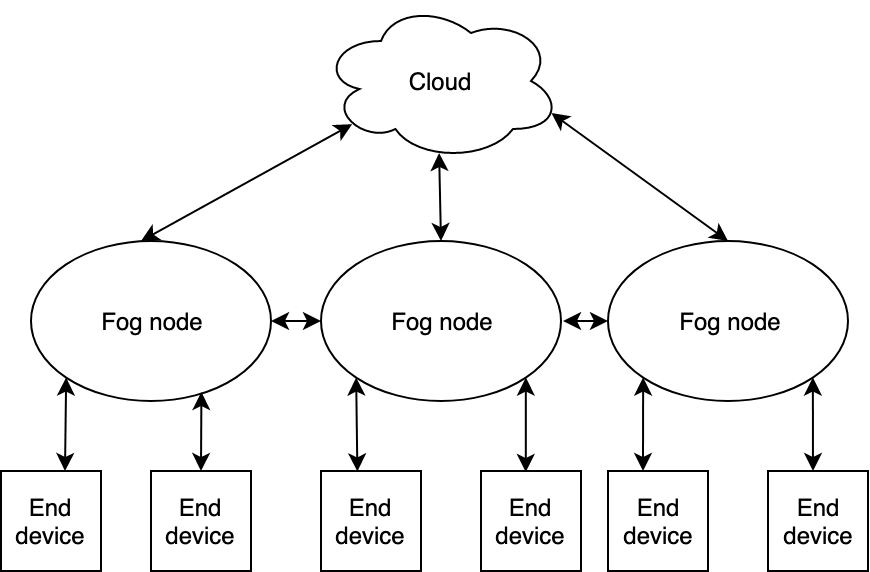
\includegraphics[width=12cm]{fog-computing-infrastructure}
    \caption{Fog infrastructure}
    \label{fig:foginfrastructure}
\end{figure}

\section{Flow-based Programming}
Flow-based programming (FBP) allows the developer to structurally define the informational flow within a system. While it is not important \textit{where} a specific task is physically executed, FBP focuses on the \textit{path} the data takes from one process to another. Any number of further processes can be involved in between, while every process manipulates or just reads the data to trigger further actions. Each process has a specific in- and output. For the developer, all execution units are \textit{black box processes}, which can consume and create data. The processes can be executed and recomposed in any order, as long as output and input formats match each others. It is also possible to split the data flow at one point and combine it back together at a later point, making parallel computation possible.\\

Data between processes is transferred in \textit{Information Packets (IPs)}. IPs belong to a single process or are in a transfer state, where they are owned by no process. As soon as a process receives an IP, it can start processing it without the need to communicate with other processes, because the IP contains all necessary information the process needs to fulfil the task. This makes FBP highly attractive for Fog computing environments, where each fog node can be used to execute one or more process types, depending on the process requirements like computation power, bandwidth or latency.

\section{QoS-aware resource allocation and scheduling}
In this section, related work on QoS, load-balancing, and resource allocation is discussed. Although fog is considered as a cloud close to the ground, load balancing strategies of cloud computing can not be directly adopted in the fog network since the heterogeneity of fog \cite{novel-load-balancing}.

\subsection{FogTorch}
In \cite{fogtorch} a model to support QoS-aware deployment of multicomponent IoT applications to a Fog infrastructures is proposed. Furthermore, a Java tool called \texttt{FogTorch} has been prototyped which implements that model. The model allows to define QoS profiles, Fog infrastructures and IoT applications, which are used to determine eligible deployments.\\

A \texttt{QoS profile} defines bandwidth and average latency required for an application, or offered by a communication link. A \texttt{fog infrastructure} includes IoT devices, Fog nodes, Cloud data centers, and communication links, while each link is associated to its QoS profile. Cloud computing is modeled according to the hypothesis that it can offer a virtually unlimited amount of hardware capabilities. An IoT \texttt{application} is a set of independently deployable components that are working together and must meet some QoS constraints. For this, software components as well as required interactions among components, including the desired QoS profile, are defined. At the end, an \texttt{eligible deployment} for the IoT application is calculated by an algorithm.\\

An algorithm selects where a component is to be deployed within the Cloud to Things continuum. For this, a preprocessing procedure which reduces the search space for eligible deployments runs before a backtracking procedure and heuristics are used to determine a single eligible deployment. Because the proposed backtracking algorithm follows a heuristic approach to get a solution faster, it shows greedy behavior.\\

\cite{fogtorchpi} presents FogTorch$\pi$, an open source prototype based on ForTorch\cite{fogtorch}. FogTorch$\pi$, compared to FogTorch, additionally allows to express \textit{processing capabilities} and average QoS attributes of a Fog infrastructure, along with processing and QoS requirements of an application, and it determines deployments of the application over the Fog infrastructure that meet all such requirements \cite{fogtorchpi}. It models the QoS of communication links by using probability distributions (based on historical data) repeatedly to simulate different runtime behaviours. At the end, it aggregates the results for deployments generated over a large number runs. The output of FogTorch$\pi$ contains eligible deployments (like FogTorch), but additionally outputs QoS assurance and resource consumption over Fog nodes which allows to compare possible deployments and evaluate the impact of possible changes.

\subsection{iFogSim}

In \cite{ifogsim} a tool called \textit{iFogSim} is designed and implemented. It is used to \textit{simulate} a fog computing environment by using two different placement strategies (\textit{cloud-only} and \textit{edge-ward}). Besides other evaluations, it was found that the average latency of a control loop is much lower in a \textit{edge-ward} than in a \textit{cloud-only}  placement strategy.\\

In this work an algorithm for a \textit{real} fog environment is developed and implemented in section \ref{cha:algorithm}, which is inspired by \textit{iFogSim} and adopts some classes of its class model. For this reason, the relevant classes for this work are briefly summarized in the following.\\

\begin{itemize}
    \item \underline{\texttt{FogDevice}}: Specifies hardware characteristics of a node like CPU power, available RAM, available disk storage, as well as network communication capabilities (uplink and downlink).
    
    \item \underline{\texttt{Sensor}}: Represents an IoT sensor, is connected to a \texttt{FogDevice}, has an \textit{output characteristic}.
    
    \item \underline{\texttt{Tuple}}: Fundamental communication unit. It is characterized by its \textit{type}, \textit{source} and \textit{destination} application module. Processing requirements (in \textit{Million Instructions}) and \textit{lenght of data} are defined as well. 
    
    \item \underline{\texttt{Application}}: An application consists of several modules, each module processing incoming data.
    \begin{itemize}
        \item \underline{\texttt{AppModule}}: Represents processing elements of an application. An instance of an \textit{AppModule} produces an output tuple for every incoming tuple.
        
        \item \underline{\texttt{AppEdge}}: Models the \textit{data-dependency} between a pair of application modules. It is characterized by the \textit{type} of a tuple, \textit{processing requirements} as well as the \textit{length of data} the tuple carries.
        
        \item \underline{\texttt{AppLoop}}: Specifies \textit{process-control loops}. A loop has a \textit{starting} and \textit{terminating} module (as well as any number of modules in between). Figure \ref{fig:apploop} shows an applications containing two loops: \begin{enumerate}
            \item \texttt{Sensor -> Analyzer -> User Interface}
            \item \texttt{Sensor -> Analyzer -> Actuator}
        \end{enumerate}
        For every loop an \textit{end-to-end latency} can be specified. For instance, the second loop might be time critital since an actuator changes the environment based on the sensors value and thus has a lower latency requirement.
    \end{itemize}
\end{itemize}

\begin{figure}
    \centering
    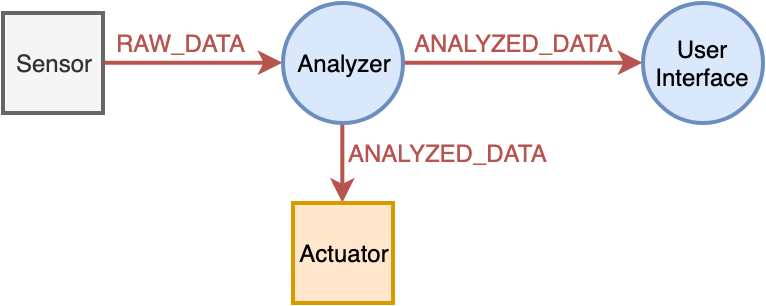
\includegraphics[width=9cm]{algorithm-apploop}
    \caption{Application containing four \texttt{AppModule} and two \texttt{AppLoop} instances}
    \label{fig:apploop}
\end{figure}

\subsection{MPSO-CO}

\cite{novel-load-balancing} proposes the \textit{modified constrained optimization particle swarm optimization} (MPSO-CO) load balancing algorithm, which is \textit{software defined networking} (SDN)-based. Compared to the \textit{constrained optimization particle swarm optimization} (PSO-CO) algorithm, which it is based on, it is able to effectively decrease latency and improve the QoS in a \textit{software defined cloud/fog networking} (SDCFN) architecture. It was developed for applications in the Internet of Vehicles (IoV) which still stuffers from high processing latency. SDN is used for centralized control and to get the required information before load balancing. The key technology of SDN is decoupling data and control plane. The controller collects real-time information of the network including load, processing speed, and communication latency. Based on that, it can formulate optimal load balancing strategies for the network. It is shown that the MPSO-CO algorithm obtains lower latency compared to PSO-CO, Max-Min load balancing algorithm (LBMM) and greedy load balancing algorithm (Greedy-LB), since LBMM and Greedy-LB don’t take the transmission latency into account, and PSO-CO may fall into the local optimum. However, on a low task load (lower than 0.05GB), where transmission latency is not a relevant factor, there is no big difference regarding the latencies of the different algorithms and they all perform pretty much the same.

\section{MAPE-K}
A self-adaptive system consists of the two layers \texttt{managed subsystem} and \texttt{managing subsystem}, whereas the managing subsystem resides on top of the managed subsystem and monitors the managed subsystem as well as the environment. It realizes a feedback loop which adapts to changes, e.g. environmental changes like congestion or failures, or to goal changes \cite{mape-k}.\\

The \textit{Monitor-Analyze-Plan-Execute over a Knowledge base} (MAPE-K) \cite{autonomic-computing} reference control model is the most influential reference control model for autonomic and self-adaptive systems. It is commonly used to realize feedback loops \cite{mape-k}.\\

The component \texttt{Knowledge} (K) is responsible for storing and providing data from/to other components. The component \texttt{Monitor} (M) collects data through probes or sensors from the environment as well as data from the managed subsystem. The collected data is saved in K. The component \texttt{Analyze} (A) analyzes the collected data to check if the system needs an adaption. If this is the case, the component \texttt{Plan} (P) will determine which actions are required to put the system in the desired state. The component \texttt{Execution} (E) then carries out these actions. \cite{mape-k}  